% xelatex
\documentclass[blue,normal,cn]{elegantnote}
\usepackage{array}
\usepackage{courier}
\usepackage{xcolor}
\usepackage{zhnumber}
\usepackage{ulem}
\usepackage{float}

\definecolor{light-gray}{gray}{0.95}
\newcommand{\code}[1]{\colorbox{light-gray}{\texttt{#1}}}
\newfontfamily\courier{Courier New}
\lstset{linewidth=1.1\textwidth,
	numbers=left,
	basicstyle=\small\courier,
	numberstyle=\tiny\courier,
	keywordstyle=\color{blue}\courier,
	commentstyle=\it\color[cmyk]{1,0,1,0}\courier, 
	stringstyle=\it\color[RGB]{128,0,0}\courier,
	frame=single,
	backgroundcolor=\color[RGB]{245,245,244},
	breaklines,
	extendedchars=false, 
	xleftmargin=2em,xrightmargin=2em, aboveskip=1em,
	tabsize=4, 
	showspaces=false
	basicstyle=\small\courier
}
\title{实验 1: MIPS 指令系统和 MIPS 体系结构}
\version{$\aleph$}
\date{\zhtoday}

\begin{document}
\author{
    \begin{tabular}[t]{cccc}
        于海鑫     & 田静悦     & 赵泉斌     & 黄震\footnote{以学号顺序排序} \\
        2017211240 & 2017211259 & 2017211268 & 2017211274
    \end{tabular}
}
\maketitle

\section{实验目的}
\begin{enumerate}
    \item 了解和熟悉指令级模拟器
    \item 熟练掌握 MIPSsim 模拟器的操作和使用方法
    \item 熟悉 MIPS 指令系统及其特点,加深对 MIPS 指令操作语义的理解
    \item 熟悉 MIPS 体系结构
\end{enumerate}

\section{实验平台}

实验平台采用指令级和流水线操作级模拟器 \code{MIPSsim}。

\section{实验内容和步骤}

首先要阅读 MIPSsim 模拟器的使用方法(见附录),然后了解 MIPSsim 的指令系统和汇编语言。

\begin{enumerate}[wide=0pt, listparindent=2em, parsep=0pt]
    \item 启动 MIPSsim(用鼠标双击 MIPSsim.exe)。
    \item 选择 “配置” $\rightarrow$ “流水方式” 选项,使模拟器工作在非流水方式下。
    \item 参照 MIPSsim 使用说明,熟悉 MIPSsim 模拟器的操作和使用方法。

          可以先载人一个样例程序(在本模拟器所在的文件夹下的“样例程序”文件夹中),然后
          分别以单步执行一条指令、执行多条指令、连续执行、设置断点等的方式运行程序,观
          察程序执行情况,观察 CPU 中寄存器和存储器的内容的变化。
    \item 选择“文件” $\rightarrow$ “载入程序” 选项,加载样例程序 \code{alltest.asm} ,然后查看 “代码” 窗口,至看程序所在的位置(起始地址为 \sout{0x00000100} \textcolor{red}{\textbf{0x00000000}})

          \begin{figure}[H]
              \centering
              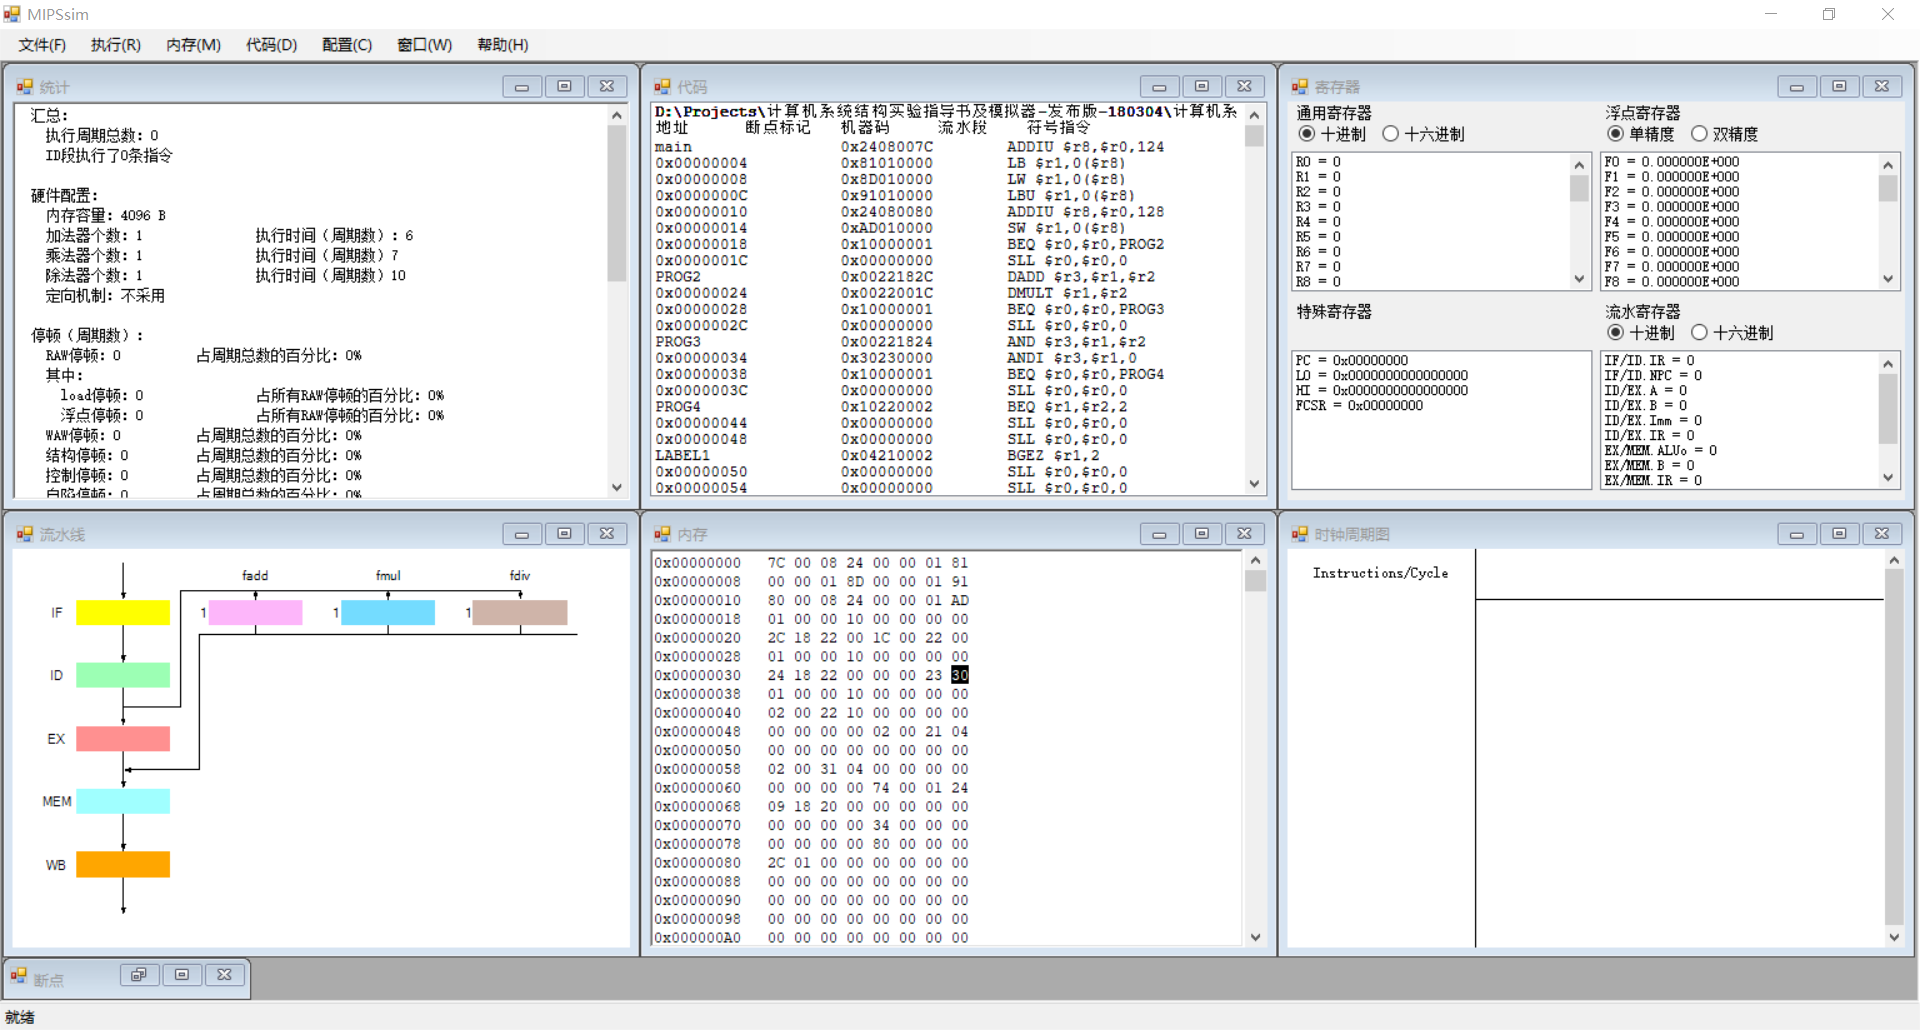
\includegraphics[width=1\textwidth]{fig/load_alltest.png}
              \caption{载入程序}
              \label{fig:load_alltest}
          \end{figure}

    \item 查看 “寄存器” 窗口 PC 寄存器的值:\textbf{[PC]} = \uline{0x00000000}。
    \item 执行 \code{load} 和 \code{store} 指令,步骤如下:

          \begin{itemize}[leftmargin=3em]
              \item 单步执行 1 条指令(F7)。
              \item 下一条指令地址为 \uline{0x00000004},是一条 \uline{有} 符号载入 \uline{字节} 指令。
              \item 单步执行 1 条指令(F7)。
              \item 查看 R1 的值,\textbf{[R1]} = \uline{0xFFFFFFFFFFFFFF80}。
              \item 下一条指令地址为 \uline{0x00000008},是一条 \uline{无} 符号载入 \uline{字} 指令。
              \item 单步执行 1 条指令(F7)。
              \item 查看 R1 的值,\textbf{[R1]} = \uline{0x0000000000000080}。
              \item 下一条指令地址为 \uline{0x0000000C},是一条 \uline{无} 符号载入 \uline{字节} 指令。
              \item 单步执行 1 条指令(F7)。
              \item 查看 R1 的值,\textbf{[R1]} = \uline{0x0000000000000080}。
              \item 单步执行 1 条指令(F7)。
              \item 下一条指令地址为 \uline{0x00000014},是一条保存 \uline{字} 指令。
              \item 单步执行 1 条指令(F7)。
              \item 查看内存 \code{BUFFER} 处字的值,值为 \uline{0x80}。(内存 $\rightarrow$ 符号表)
          \end{itemize}

    \item 执行逻辑运算类指令。步骤如下:
          \begin{itemize}[leftmargin=3em]
              \item 双击 “寄存器” 窗口中的 R1,将其值修改为 2
                    。
              \item 双击 “寄存器” 窗口中的 R2,将其值修改为 3
              \item 单步执行 1 条指令。
              \item 下一条指令地址为 \uline{0x00000020},是一条加法指令。
              \item 单步执行 1 条指令。
              \item 查看 R3 的值,\textbf{[R3]} = \uline{0x0000000000000005}。
              \item 下一条指令地址为 \uline{0x00000024},是一条乘法指令。
              \item 单步执行 1 条指令。
              \item 查看 L0、HI 的值,\textbf{[LO]}= \uline{0x0000000000000006},\textbf{[HI]}= \uline{0x0000000000000000}。
          \end{itemize}

    \item 执行逻辑运算类指令。步骤如下:

          \begin{itemize}[leftmargin=3em]
              \item 双击 “寄存器” 窗口中的 R1,将其值修改为 0xFFFF0000。
              \item 双击 “寄存器” 窗口中的 R2,将其值修改为 0xFF00FF00。
              \item 单步执行 1 条指令。
              \item 下一条指令地址为 \uline{0x00000030},是一条逻辑与运算指令,第二个操作数寻址方式是 \uline{寄存器直接寻址}。
              \item 单步执行 1 条指令。
              \item 查看 R3 的值,\textbf{[R3]} = \uline{0x00000000FF000000}。
              \item 下一条指令地址为 \uline{0x00000034},是一条逻辑与运算指令,第二个操作数寻址方式是 \uline{立即数寻址}。
              \item 单步执行 1 条指令。
              \item 查看 R3 的值,\textbf{[R3]} = \uline{0x0000000000000000}。
          \end{itemize}
    \item 执行控制转移类指令。步骤如下:
          \begin{itemize}[leftmargin=3em]
              \item 双击 “寄存器” 窗口中的 R1,将其值修改为 2
                    。
              \item 双击 “寄存器” 窗口中的 R2,将其值修改为 2
              \item 单步执行 1 条指令。
              \item 下一条指令地址为 \uline{0x00000040},是一条 BEQ 指令,其测试条件是 \uline{\$r1 == \$r2},目标地址为 \uline{0x0000004C}。
              \item 单步执行 1 条指令。
              \item 查看 PC 的值,\textbf{[PC]}= \uline{0x0000004C},表明分支 \uline{成功}。
              \item 下一条指令是一条 BGEZ 指令,其测试条件是 \uline{\$r1 $\geq 0$},目标地址为 \uline{0x00000058}。
              \item 单步执行 1 条指令。
              \item 查看 PC 的值,\textbf{[PC]}= \uline{0x00000058},表明分支 \uline{成功}。
              \item 下一条指令是一条 BGEZAL 指令,其测试条件是 \uline{\$r1 $\geq 0$},目标地址为 \uline{0x00000064}。
              \item 单步执行 1 条指令。
              \item 查看 PC 的值,\textbf{[PC]}= \uline{0x00000064},表明分支 \uline{成功};查看 R31 的值,\textbf{[R31]} = \uline{0x0000005C}。
              \item 单步执行 1 条指令。
              \item 查看 R1 的值,\textbf{[R1]} = \uline{0x0000000000000074}。
              \item 下一条指令地址为 \uline{0x00000068},是一条 JALR 指令,保存目标地址的寄存器为 R\uline{1},保存返回地址的目标寄存器为 R\uline{3}。
              \item 单步执行 1 条指令。
              \item 查看 PC 和 R3 的值,\textbf{[PC]}= \uline{0x00000074},[R3]=\uline{0x000000000000006C}。
          \end{itemize}
          \begin{figure}[H]
              \centering
              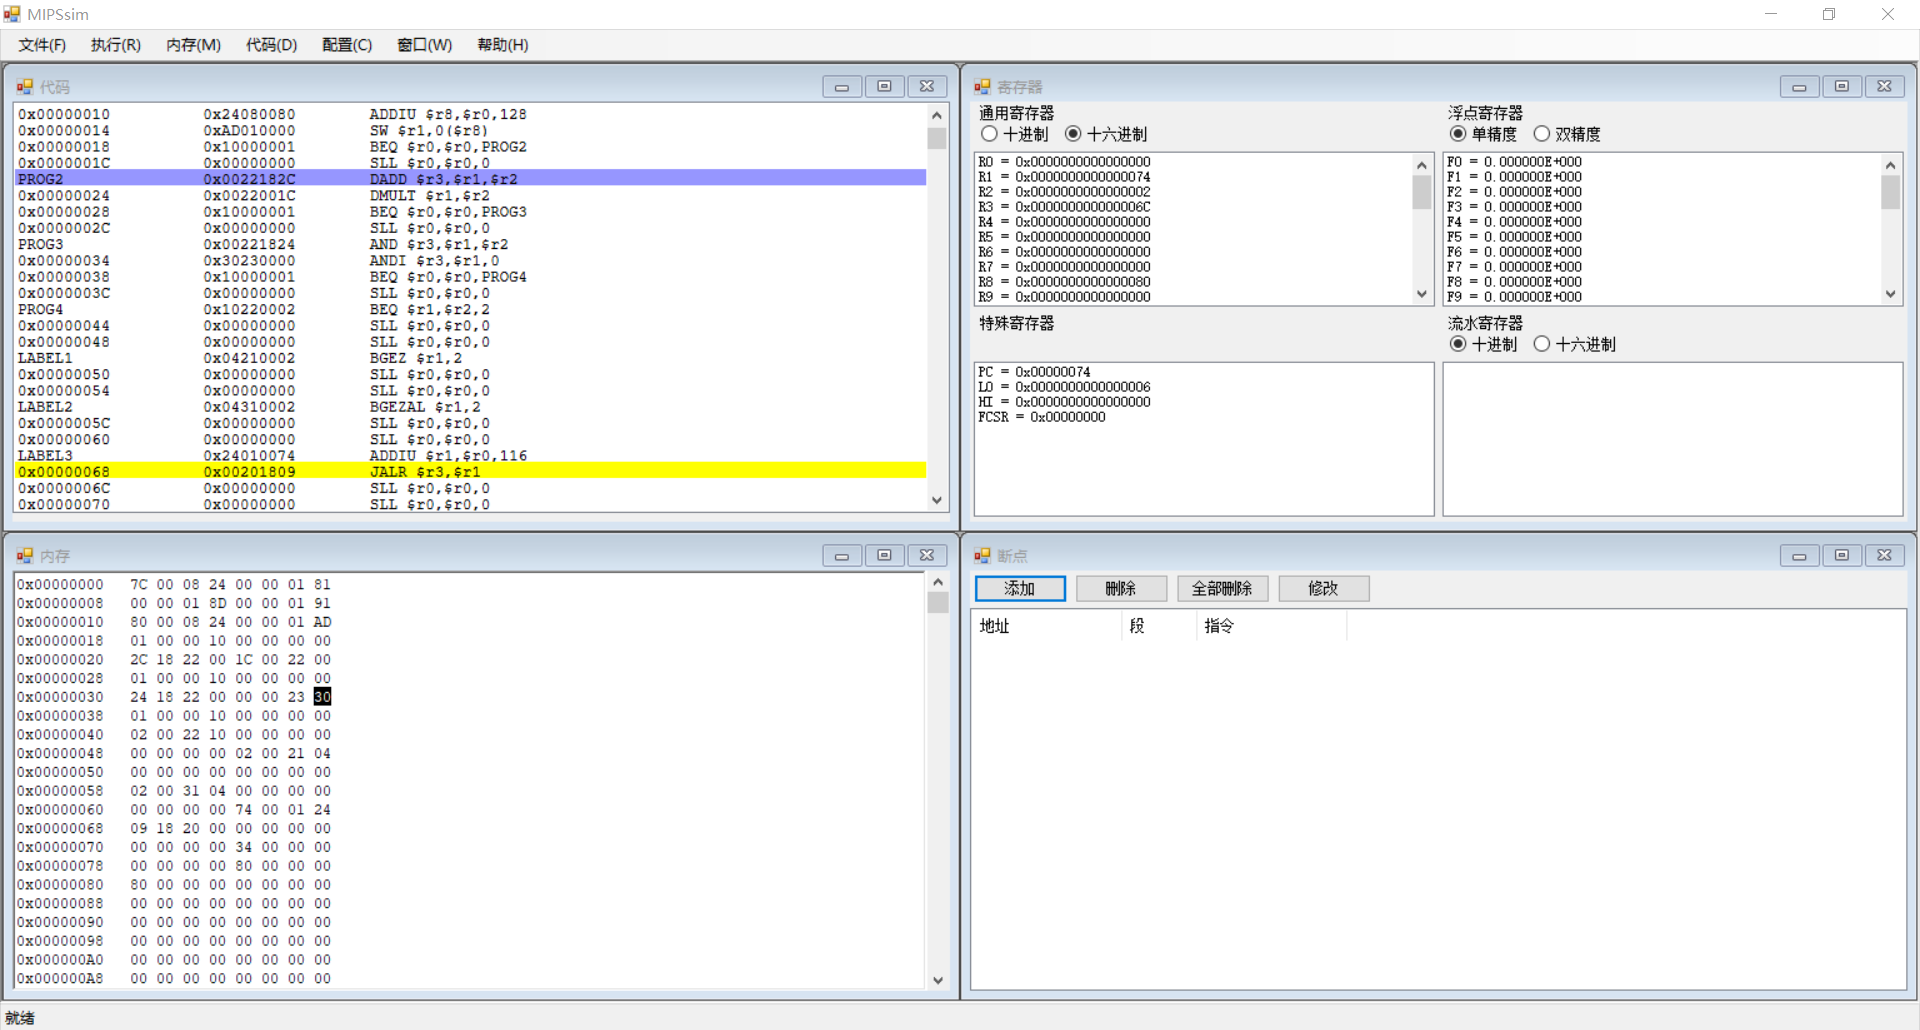
\includegraphics[width=1\textwidth]{fig/fin_alltest.png}
              \caption{程序运行完成}
              \label{fig:fin_alltest}
          \end{figure}
\end{enumerate}

\section{实验中的问题与心得}

本次实验主要目的是在于熟悉模拟器的使用以及了解 MIPS 体系结构的特点,实验中没有遇到任何问题。

至于心得,个人认为本次实验中的填空过于繁琐,PC 的位置无需重复确认,其行为在 MIPS 的手册上有着明确定义,只通过展示正常情况下的 PC 变化以及发生跳转时 PC 的变化即可使得同学们较好的了解和把握 MIPS 体系结构的特点。同理,对于指令作用的重复提问也很繁琐且没有必要。再就是实验指导书上出现了一些很明显的错误,比如在前文中以红色粗体标出的 \code{.text} 段的起始位置的错误,再比如前面的 \code{MIPSsim} 的使用手册上出现了实际程序中根本不存在的选项。这些只要实际做了一次实验都会发现的问题依然存在说明实验指导书的编撰过程中依然存在一些不严谨的地方,希望能够在下一学年时能够进行修正。

\end{document}